\documentclass[diss,capa]{texufpel}

\usepackage{subfigure}
\usepackage{todo}
\usepackage{xcolor, colortbl, color}
\usepackage{tikz}
\usepackage{verbatim}
\usepackage{pgfplots}

\usepackage[utf8]{inputenc} % acentuacao
\usepackage{graphicx} % para inserir figuras
\usepackage[T1]{fontenc}

\hypersetup{
    hidelinks, % Remove coloração e caixas
    unicode=true,   %Permite acentuação no bookmark
    linktoc=all %Habilita link no nome e página do sumário
}

\unidade{Centro de Desenvolvimento Tecnológico}
\programa{Programa de Pós-Graduação em Computação}
\curso{Ciência da Computação}

\unidadeeng{Technology Development Center}
\programaeng{Postgraduate Program in Computing}
\cursoeng{Computer Science}

\title{Escalonador de Transações para Arquiteturas NUMA}

\author{Costa}{Michael Alexandre}
\advisor[Prof.~Dr.]{Du Bois}{André}
% \coadvisor[Prof.~Dr.]{Aguiar}{Marilton Sanchotene de}
% \collaborator[Prof.~Dr.]{Aguiar}{Marilton Sanchotene de}

%Palavras-chave em PT_BR
\keyword{Memórias Transacionais - TM}
\keyword{Non-Uniform Memory Access - NUMA}
\keyword{Escalonador}
% \keyword{}

%Palavras-chave em EN_US
\keywordeng{Transactional Memory - TM}
\keywordeng{Non-Uniform Memory Access - NUMA}
\keywordeng{Scheduler}
% \keywordeng{}

\begin{document}

%\renewcommand{\advisorname}{Orientadora}           %descomente caso tenhas orientadora
%\renewcommand{\coadvisorname}{Coorientadora}      %descomente caso tenhas coorientadora

\maketitle 

\sloppy

\fichacatalografica

%Composição da Banca Examinadora
% \begin{aprovacao}{30 de fevereiro de 2019} %data da banca por extenso
%   \noindent Prof. Dr. Marilton Sanchotene de Aguiar (orientador)\\
%   Doutor em Computação pela Universidade Federal do Rio Grande do Sul.\\[1cm]

%   \noindent Prof. Dr. Paulo Roberto Ferreira Jr.\\
%   Doutor em Computação pela Universidade Federal do Rio Grande do Sul.\\[1cm]

%   \noindent Prof. Dr. Ricardo Matsumura Araujo\\
%   Doutor em Computação pela Universidade Federal do Rio Grande do Sul.\\[1cm]

%   \noindent Prof. Dr. Luciano da Silva Pinto\\
%   Doutor em Biotecnologia pela Universidade Federal de Pelotas.
% \end{aprovacao}

%Opcional
\begin{dedicatoria}
  Dedico\ldots 
\end{dedicatoria}

%Opcional
\begin{agradecimentos}
  Agradeço\ldots 
\end{agradecimentos}

%Opcional
\begin{epigrafe}
  Só sei que nada sei.\\
  {\sc --- Sócrates}
\end{epigrafe}

%Resumo em Portugues (no maximo 500 palavras)
\begin{abstract}
...
\end{abstract}

%Resumo em Inglês (no maximo 500 palavras)
\begin{englishabstract}{Transaction Scheduler for NUMA Architectures}
...
\end{englishabstract}

%Lista de Figuras
\listoffigures

%Lista de Tabelas
\listoftables

%lista de abreviaturas e siglas
\begin{listofabbrv}{ABNT}%coloque aqui a maior sigla para ajustar a distância
        \item[TM] Memórias Transacionais
        \item[STM] Memórias Transacionais em Software
        \item[NUMA] Non-Uniform Memory Access
        \item[UMA] Uniform Memory Access
\end{listofabbrv}

%Sumario
\tableofcontents

\chapter{Introdução}

\section{Motivação}
...~\cite{vonNeumann:1966:TSR}.

\section{Objetivos}

...~\ref{tabela}.

\begin{table}
  \begin{center}
    \caption{Nome da Tabela}\label{tabela}
    \begin{tabular}{p{4cm}p{5cm}p{6cm}}
      \hline
      Blabla & Blabla & Blablabla\\
      \hline
      {\small Bla} & {\small Blabla} & {\small\em Bla blabla blablabla blabla
        blablabla blabla blablabla.}\\
      {\small Bla} & {\small Blabla} & {\small\em Bla blabla blablabla blabla
        blablabla blabla blablabla.}\\
      {\small Bla} & {\small Blabla} & {\small\em Bla blabla blablabla blabla
        blablabla blabla blablabla.}\\
      {\small Bla} & {\small Blabla} & {\small\em Bla blabla blablabla blabla
        blablabla blabla blablabla.}\\
      {\small Bla} & {\small Blabla} & {\small\em Bla blabla blablabla blabla
        blablabla blabla blablabla.}\\
      {\small Bla} & {\small Blabla} & {\small\em Bla blabla blablabla blabla
        blablabla blabla blablabla.}\\
      \hline
    \end{tabular}
  \end{center}
\end{table}

\subsection{Objetivo geral}

...

\subsection{Objetivos especificos}

\begin{itemize}

  \item ...; e
  \item ...
\end{itemize}

\section{Estrutura do Texto}

...
Teste do overleaf.
...

\chapter{Memórias Transacionais}
\label{chapter::stm}

Memória Transacional, ou \emph{Transactional Memory}~(TM), é uma classe de mecanismos de sincronização que fornece uma execução atômica e isolada de alterações em um conjunto de dados compartilhados. Estas estão sendo desenvolvidas para que no futuro tornem-se o principal meio de fazer a sincronização em um programa concorrente, substituindo a sincronização baseada em \emph{locks}~\cite{energyawaretm}. As TMs podem ser implementadas em \emph{software} (STM), em \emph{hardware} (HTM) ou ainda em uma versão híbrida de \emph{hardware} e \emph{software}.

Na programação utilizando STMs, todo o acesso à memória compartilhada é realizado dentro de transações e todas as transações são executadas atomicamente em relação a transações concorrentes.

A principal vantagem na programação usando STM é que o programador apenas delimita as seções criticas e não é necessário preocupar-se com a aquisição e liberação de \emph{locks}. Os \emph{locks}, quando utilizados de forma incorreta, podem levar a problemas como \emph{deadlocks}~\cite{BAND10}.

\section{Propriedades}

Transação é uma sequência finita de escritas e leituras na memória executada por uma \emph{thread}~\cite{herlihy93}, e deve satisfazer três propriedades:

\begin{itemize}
 \item \textbf{Atomicidade}: cada transação faz uma sequência de mudanças provisórias na memória compartilhada. Quando a transação é concluída, pode ocorrer um \emph{commit}, tornando suas mudanças visíveis a outras \emph{threads} instantaneamente, ou pode ocorrer um \emph{abort}, fazendo com que suas alterações sejam descartadas;

 \item \textbf{Consistência}: as transações devem garantir que um sistema consistente deve ser mantido consistente. Esta propriedade esta relacionada com o conceito de invariância;

 \item \textbf{Isolamento}: as transações não interferem nas execuções de outras transações, assim parecendo que elas são executadas serialmente. Uma transação não observa o estado intermediário de outra.
\end{itemize}

\section{Versionamento de Dados}

O versionamento de dados faz é responsável pelo gerenciamento das versões dos dados. Ele armazena tanto o valor do dado no início de uma transação como também o valor do dado modificado durante a transação, isso para garantir a propriedade de atomicidade~\cite{BaldassinTese2009}.

\begin{figure}[!htp]
\centering
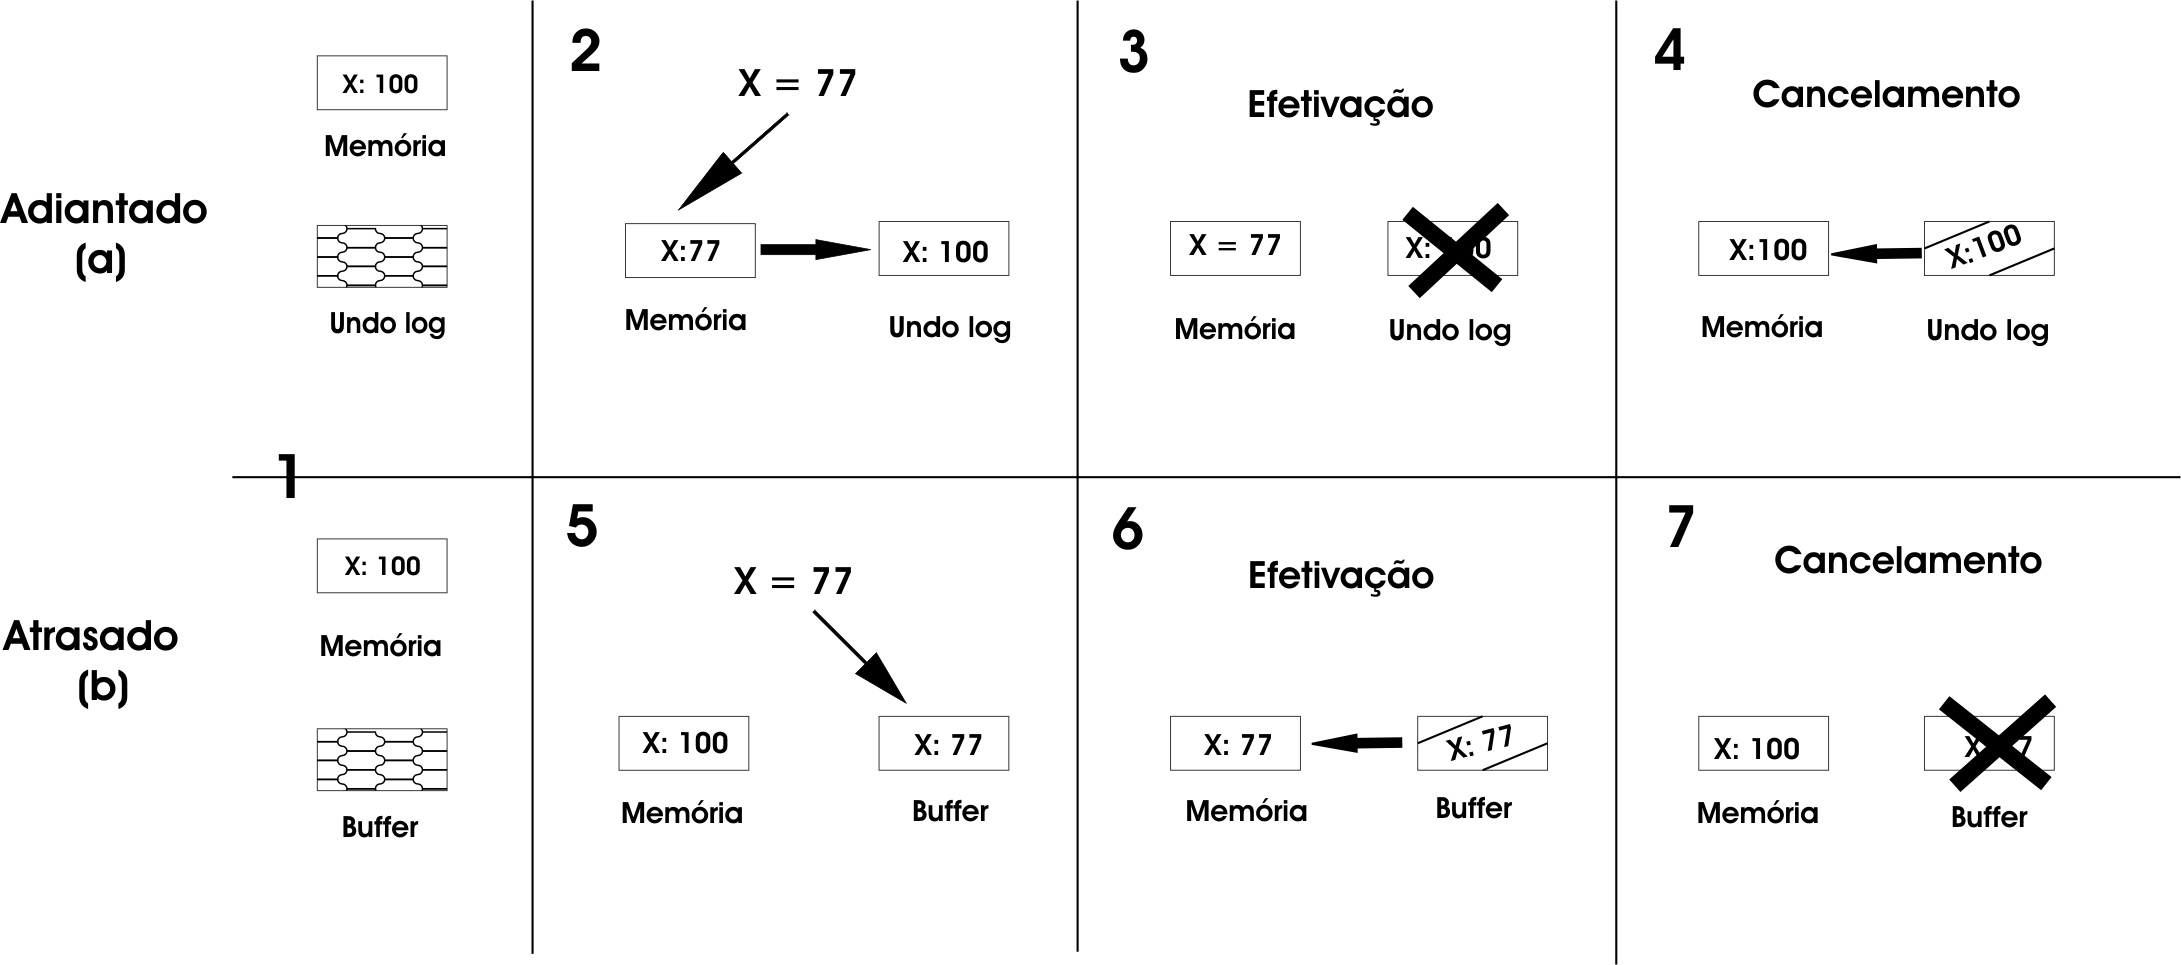
\includegraphics[height=7cm]{images/versionamento.png}
\caption{Exemplo de versionamento adiantado (a) e atrasado (b). Fonte:~\cite{BaldassinTese2009}}
\label{figuraversionamento}
\end{figure}

Existem dois tipos de versionamento de dados:

\begin{itemize}
 \item \textbf{Versionamento Adiantado}: como pode ser visto na Figura~\ref{figuraversionamento}~(a), o valor modificado durante a transação é armazenado direto na memória e o valor inicial é armazenado em um \emph{undo log}, para que no caso de cancelamento na transação o valor inicial seja restaurado na memória.

 \item \textbf{Versionamento Atrasado}: como pode ser visto na Figura~\ref{figuraversionamento}~(b) neste versionamento o valor modificado durante a transação é armazenado em um \emph{buffer} e o valor inicial é mantido na memória até que aconteça um \emph{commit} na transação, onde o valor armazenado no \emph{buffer} é escrito na memória. Caso aconteça o cancelamento na transação, o valor do \emph{buffer} é descartado.
\end{itemize}

\section{Detecção de Conflito}

Mecanismos de detecção de conflitos verificam a existência de operações conflitantes durante uma transação. Um conflito ocorre quando duas transações estão acessando um mesmo dado na memória e pelo menos uma das transações está fazendo uma operação de escrita~\cite{BaldassinTese2009}.

Da mesma forma que o versionamento de dados, a detecção de conflito também pode ser de dois tipos:

\begin{itemize}
 \item \textbf{Detecção de Conflitos Adiantado}: ocorrem no momento em que duas transações acessam um mesmo dado e uma delas faz uma operação de escrita. Essa operação de escrita é detectada e então uma transação é abortada. Neste tipo de detecção pode ocorrer um problema chamado de \emph{livelock}, quando duas transações ficam cancelando-se, desta forma, a execução do programa não progride. A Figura~\ref{figuradeteccaoadiantado} mostra como é feita a detecção de conflitos adiantado.

 O Caso~1, mostra a execução sem conflitos, onde as duas transações são executadas sem problemas. Já o Caso~2, mostra o que acontece quando ocorre um conflito, onde T1 lê A e logo depois T2 escreve em A, então o conflito é detectado e T1 é abortada, após ser efetivada T2, a transação T1 consegue ler A sem problema de conflito. Por fim o Caso~3 mostra a situação de \emph{livelock}, onde as duas transações tentam ler e escrever em A, assim as duas acabam sempre se abortando.

\begin{figure}[!htp]
\centering
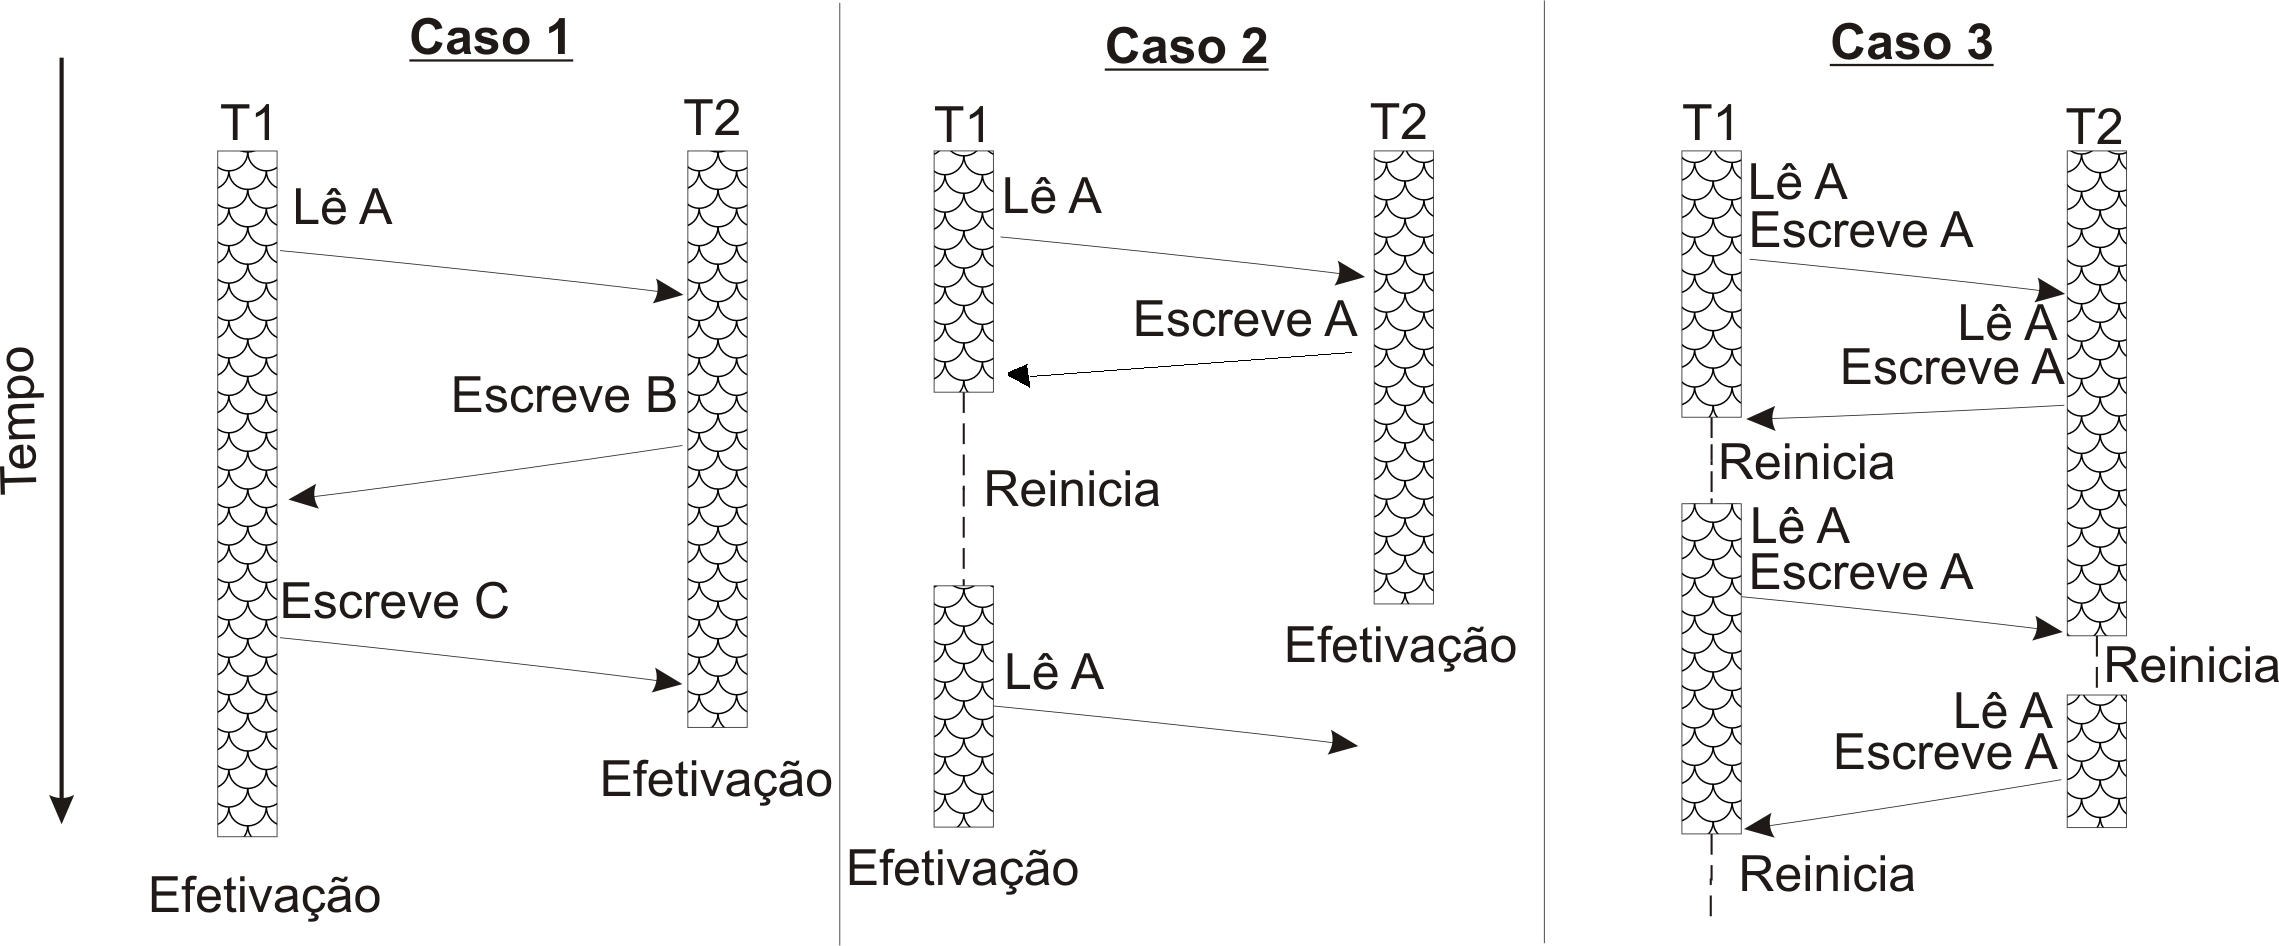
\includegraphics[height=6.5cm]{images/conflitoadiantado.png}
\caption{Detecção de conflitos em modo adiantado. Fonte:~\cite{rigotm}}
\label{figuradeteccaoadiantado}
\end{figure}


 \item \textbf{Detecção de Conflitos Atrasado}: Este tipo de detecção de conflito ocorre no final da transação.  Antes da transação ser efetuada, é verificado se ocorreu um conflito. Caso tenha ocorrido, a transação é cancelada, senão é efetivada. Para transações muito grandes não é recomendado este tipo de detecção, pois uma transação grande pode ser abortada várias vezes por transações pequenas, assim gastando tempo de processamento desnecessário, este problema se chama \emph{starvation}. A Figura~\ref{figuradeteccaoatrasado} mostra como é feita a detecção de conflitos atrasado.

 O Caso~1, mostra as transações acessando dados diferentes, não ocasionando conflitos. No Caso~2, T2 lê A que é escrita por T1. A T2 só nota o conflito quando T1 é efetivado. Logo depois de notar o conflito T2 é abortada. No Caso~3 não ocorre nenhum conflito, pois T1 lê A antes de T2 escrever. O Caso~4 mostra a situação em que, após ser cancelada, T1 volta a executar.
\end{itemize}

\begin{figure}[!htp]
\centering
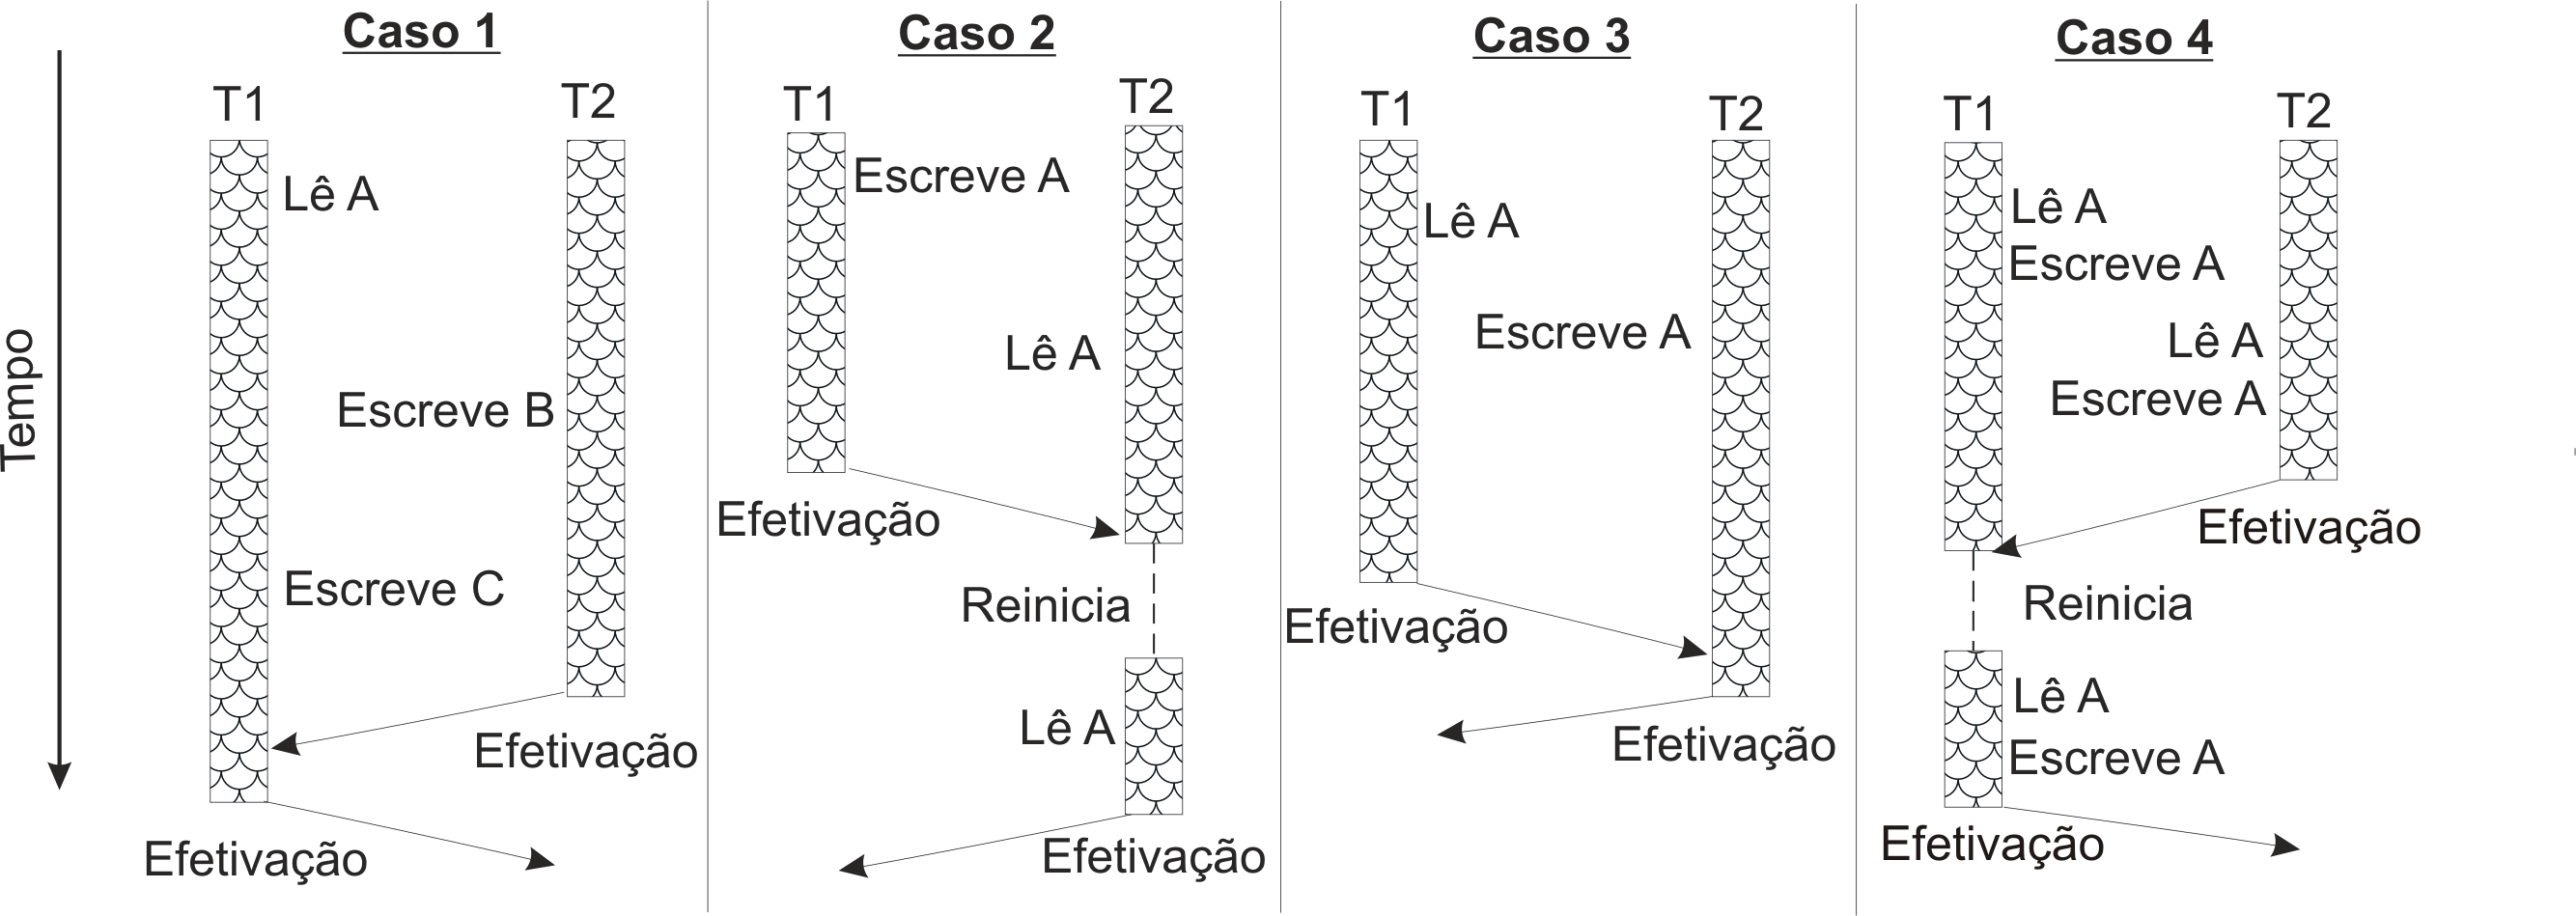
\includegraphics[height=6.5cm]{images/conflitoatrasado.png}
\caption{Detecção de conflitos em modo atrasado. Fonte:~\cite{rigotm}}
\label{figuradeteccaoatrasado}
\end{figure}


Para solucionar o problema de qual transação continuará executando, quando ocorre um conflito, é utilizado um gerenciador de contenção~\cite{TM2010}. O gerenciador de contenção é o responsável por decidir quando e qual transação vai ser abortada, isso para garantir que a execução do programa prossiga sem problemas.


\chapter{TinySTM}
\label{chapter::tiny}

A \emph{TinySTM}~\cite{TINY} é uma implementação de STM para as linguagens C e C++. Seu algoritmo é baseado em outros algoritmos de STM como o TL2~(\emph{Transactional Locking} 2)~\cite{tl2}. Ela é uma biblioteca utilizada para escrever aplicativos que usam memórias transacionais para sincronização, em substituição aos tradicionais \emph{locks}.

\section{Sincronização e Versionamento}

Na \emph{TinySTM} a sincronização é feita a partir de um \emph{array} de \emph{locks} compartilhado que gerencia o acesso concorrente à memória. Cada \emph{lock} é do tamanho de um endereço da arquitetura~\cite{TINY}, e bloqueia vários endereços de memória. O mapeamento é feito por meio de uma função \emph{hash}. A Figura~\ref{figurasincronisacaotinystm} apresenta as estruturas de dados utilizadas nesta implementação.

\begin{figure}[!htp]
\centering
\includegraphics[height=8cm]{images/tinystm.png}
\caption{Estruturas de dados utilizadas na \emph{tinySTM}. Fonte:~\cite{TINY}}
\label{figurasincronisacaotinystm}
\end{figure}

O bit menos significativo é utilizado para indicar se o \emph{lock} está em uso. Se o bit menos significativo indicar que o \emph{lock} não está em uso, nos bits restantes são armazenados um número de versão que corresponde ao \emph{commit timestamp} da transação que escreveu por último em um dos locais de memória abrangidos pelo \emph{lock}.

Se o bit menos significativo indica que o \emph{lock} está em uso, então nos bits restantes é armazenado um endereço que identifica a transação que está utilizando o dado~(isso utilizando o versionamento adiantado), ou uma entrada no \emph{write set} da transação que está utilizando o dado~(isso utilizando o versionamento atrasado). Em ambos os casos os endereços apontam para uma estrutura que é \emph{word-aligned} e seu bit menos significativo é sempre zero, por isso, o bit menos significativo pode ser utilizado como bit de bloqueio.

Quando utilizado o versionamento atrasado, o endereço armazenado no \emph{lock} permite uma operação rápida para localizar as posições de memória atualizadas abrangidas pelo \emph{lock}, no caso de serem acessados novamente pela mesma transação. Em contraste, a TL2 deve verificar o acesso à memória se a transação atual ainda não escreveu neste endereço, o que pode ser caro quando \emph{write sets} são grandes. A leitura depois da escrita não é um problema quando é utilizado o versionamento adiantado porque a memória sempre contém o último valor escrito na memória pela transação ativa.

A \emph{tinySTM} apresenta três estratégias de versionamento distintas que podem ser utilizadas, sendo que duas utilizam versionamento atrasado~(write-back) e uma utiliza versionamento adiantado~(write-through), estas são:

\begin{itemize}
 \item \textbf{Write\_Back\_ETL}: esta estratégia implementa o versionamento atrasado com \emph{encounter-time locking}, isso é, o \emph{lock} é adquirido após ocorrer uma operação de escrita e atualiza o \emph{buffer}. O valor é escrito na memória no momento do \emph{commit} da transação;

 \item \textbf{Write\_Back\_CTL}: esta estratégia implementa o versionamento atrasado com \emph{commit-time locking},isto é, ele adquire o \emph{lock} antes de ocorrer o um \emph{commit} e atualizar o \emph{buffer}. Assim como no \emph{Write-Back-ETL} o valor é escrito na memória no momento do \emph{commit} da transação;

 \item \textbf{Write\_Through}: esta estratégia implementa o versionamento adiantado com \emph{encounter-time locking}, isto é, o valor é escrito direto na memória e mantém um \emph{undo log}, caso ocorra um \emph{abort} na transação é possível restaurar o valor anterior na memória.
\end{itemize}

A \emph{TinySTM} utiliza \emph{Write\_Back\_ETL} como sua estratégia de versionamento padrão.

\section{Escritas}

Quando ocorre uma escrita em um local da memória, a transação primeiro identifica o \emph{lock} correspondente ao endereço de memória e lê o valor. Se o \emph{lock} está em uso a transação verifica se é a proprietária do \emph{lock} utilizando o endereço armazenado nos restantes bits de entrada. Caso a transação seja a proprietária então ela simplesmente escreve o novo valor e retorna. Caso contrário, a transação pode esperar por algum tempo ou abortar imediatamente. A \emph{TinySTM} utiliza a última opção como padrão em sua implementação.

Se o \emph{lock} não está em uso, a transação tenta adquiri-lo para escrever o novo valor na entrada utilizando uma operação atômica \emph{compare-and-swap}. A falha indica que outra transação adquiriu o \emph{lock} nesse meio tempo, então a transação é reiniciada.


\section{Leituras}

Quando ocorre uma leitura na memória, a transação deve verificar se o \emph{lock} está em uso ou se  o valor já foi atualizado concorrentemente por outra transação. Para esse fim, a transação lê o \emph{lock} correspondente ao endereço de memória. Se o \emph{lock} não tem proprietário e o valor~(número de versão) não foi modificado entre duas leituras, então o valor é consistente.

\section{Gerenciamento de Memória}

A \emph{TinySTM} utiliza um gerenciador de memória que possibilita qualquer código transacional utilizar memória dinâmica. As transações mantém o endereço da memória alocada ou liberada. A alocação de memória é automaticamente desfeita quando a transação é abortada, já a liberação não pode ser desfeita antes do \emph{commit}. Contudo uma transação pode somente liberar memória depois de adquirir todos os \emph{locks}, assim, um \emph{free} é semanticamente equivalente a uma atualização.

\section{Gerenciador de Contenção}

A \emph{TinySTM} implementa quatro estratégias de gerenciador de contenção, estas são:

\begin{itemize}
 \item \textbf{CM\_Suicide}: nesta estratégia a transação que detecta o conflito é abortada imediatamente;

 \item \textbf{CM\_Delay}: esta estratégia assemelhasse a \emph{CM\_Suicide}, porem, espera até que a transação que gerou o \emph{abort} tenha liberado o \emph{lock}, então reinicia a transação. Isto porque por intuição a transação a transação que foi abortada irá tentar adquirir o mesmo \emph{lock} novamente, provavelmente falhando em mais de uma tentativa. Está estratégia aumenta as chances de que a transação tenha sucesso sem gerar um grande número de \emph{aborts}, melhorando o tempo de execução do processador;

 \item \textbf{CM\_Backoff}: também parecida com a \emph{CM\_Suicide}, esta estratégia espera um tempo randômico para reiniciar a transação. Este tempo de espera é escolhido ao uniformemente ao acaso em um intervalo cujo tamanho aumenta exponencialmente a cada reinicialização;

 \item \textbf{CM\_Modular}: esta estratégia implementa vários gerenciadores de contenção, que são alternados durante a execução. Os gerenciadores utilizados são:

    \begin{itemize}
       \item \textbf{Suicide}: a transação que descobriu o conflito é abortada;

       \item \textbf{Aggressive}: é o inverso da \emph{Suicide}, a transação abortada é a outra e não a que descobriu o conflito;

       \item \textbf{Delay}: a mesma que a \emph{Suicide}, mas aguarda pela resolução do conflito para reiniciar a transação;

       \item \textbf{Timestamp}: a transação mais nova é abortada.
    \end{itemize}

\end{itemize}

A \emph{TinySTM} utiliza a \emph{CM\_Suicide} como sua estratégia padrão de gerenciamento de contenção.



\chapter{Escalonadores}

O uso de escalonadores provem melhorias nas execuções de programas, pode-se utilizar escalonadores de tarefas para melhorar o desempenho de arquiteturas, como visto no trabalho \cite{Rodolfo:2014}, consegue-se utilizar um escalonador para reduzir a latência de acesso à memória pelo processador em arquiteturas \emph{NUMA}.

Em STM o uso de escalonadores pode reduzir o número de conflitos gerados pelo aumento do paralelismo, em \cite{Nicacio2012} foi proposto um escalonador de transações dinâmico denominado \emph{LUTS}, este apresenta heurísticas de detecção de conflitos para que o escalonador de transações evite \emph{aborts} no decorrer de sua execução.

%\section{Heurísticas}

%Existem muitas heurísticas diferentes para prever conflitos, estas podem servir como base para o escalonamento de transações. Nesta seção será apresentado alguns trabalhos com heurísticas distintas.

Escalonadores fornecem diferentes abordagens para cada problema proposto, estas distintas abordagens permitem aos desenvolvedores explorar heurísticas de escalonamento que se adaptam a arquitetura utilizada propiciando uma solução mais eficiente. Para este trabalho foram estudados algumas heurísticas que serviram como base para o escalonamento de transações, estes trabalhos são:

\section{Categorias}

Di zando apresenta uma categorização dos escalonadores de STM, onde ele classifica os algoritmos de acordo com as heurísticas apresentadas por eles.

Está classificação é dividica por Baseada em Heurística e Baseado em Modelo.

\begin{itemize}
	\item Baseado em Heurística:
	\begin{itemize}
	    \item Feedback;
	    \item Predição;
	    \item Reativo; e
	    \item Heurística Mista.
	\end{itemize}
	\item Baseado em Modelo:
	\begin{itemize}
	    \item Aprendizado de Máquina;
	    \item Modelo Analítico; e
	    \item Modelo Misto.
	\end{itemize}
\end{itemize}

A tabela~\ref{tab:compare} apresenta a caracterização dos algoritmos revizados na bibliografia

\begin{table}[]
\footnotesize
\centering
\caption{Algoritmos e técnicas de escalonamento}
\label{tab:compare}
\begin{tabular}{l|l}
\hline
Escalonador & Técnica \\ \hline
ATS & Feedback \\
Probe & Feedback \\
F2C2 & Feedback \\
Shrink & Predição \\
SCA & Predição \\
CAR-STM & Reativo \\
RelSTM & Reativo \\
LUTS & Heurística Mista \\
ProVIT & Heurística Mista \\
SAC-STM & Aprendizado de Máquina \\
CSR-STM & Modelo Analítico \\
MCATS & Modelo Analítico \\
AML & Modelo Misto \\
\hline
\end{tabular}
\end{table}

\subsection{ATS}

\emph{Adaptive Transaction Scheduling}~(ATS)~\cite{ats2008} apresenta uma lista global onde é inserida todas transações conflitantes, assim o escalonador garante que será executada apenas uma transação por vez.

\subsection{Blake}

\emph{Blake}~\cite{blake2009} apresenta um escalonador proativo com gerenciamento de conflito, esta previsão ocorre através do armazenamento de um valor de confiança que indica a probabilidade de ocorrência do conflito, assim, o escalonador utiliza do valor de confiança para decidir entre executar a transação, esperar ou executar outra transação.

\subsection{CAR-STM}

\emph{CAR-STM}~\cite{carstm2008} mantém uma fila e uma \emph{thread} para cada núcleo disponível na máquina, o escalonador seleciona uma das filas e insere a transação que esta prestes a iniciar, após isto, passa o controle para a \emph{thread} na qual esta fila pertence. A idéia principal é que durante o tempo de execução o escalonador insira as transações abortadas na fila da transação conflitante, assim, reduzindo o número de \emph{aborts} através da serialização destas transações.

\subsection{LUTS}

\emph{LUTS} apresenta um escalonador de transações em nível de usuário, este apresenta uma heurística proativa que usa o escalonador para evitar o início de transações conflitantes, escolhendo na fila de tarefas uma transação menos suscetível ao conflito.

\subsection{Shirink}

\emph{Shirink}~\cite{shirink2009} é uma técnica de detecção de conflitos, este evita inicializar transações com maiores chances de \emph{abort}. Esta previsão toma como base os acessos realizados anteriormente pelas transações, porém a técnica é ativada depois que um determinado número de \emph{aborts} ocorram, assim, evitando \emph{overhead} de execução.

\chapter{Arquiteturas}
\label{chapter::arquiteturas}

Dependendo da localização física da memória em relação aos processadores, o tempo de acesso a uma posição de memória pode ser uniforme ou não. Surge então as arquiteturas denominadas de \emph{UMA~(Uniform Memory Access)} e \emph{NUMA~(Non Uniform Memory Access)} \cite{carissimi_2007}.

Máquinas \emph{NUMA} tem a vantagem de agregar maior paralelismo ao adicionar mais processadores sem aumentar o número de conflitos e o gargalo de acesso ao barramento. Sua arquitetura é feita para que os processadores não utilizem o mesmo barramento de acesso à memória como é feito em arquiteturas \emph{UMA}. %, a sua  principal característica é o tempo não uniforme de acesso à memória

As arquiteturas \emph{NUMA} possuem múltiplos núcleos dispostos em conjuntos de processadores (Nodos), a memória é fisicamente composta por vários bancos de memória, podendo estar cada um deles vinculados a um Nodo e a um espaço de endereçamento compartilhado. Nesse caso, quando o processador acessa à memória que está vinculada a si, diz-se que houve um acesso local. Se o acesso for à memória de outro processador, diz-se que ocorreu um acesso remoto.

Os acessos remotos são mais lentos que os acessos locais, uma vez que é necessário passar pela rede de interconexão para que se consiga chegar ao dado localizado na memória remota \cite{Rodolfo:2014}. A Figura~\ref{arquiteturas_config} ilustra de maneira genérica, \ref{uma_fig} uma máquina de arquitetura \emph{UMA} e \ref{numa_fig} uma máquina de arquitetura \emph{NUMA}. Pode-se observar que, na arquitetura \emph{UMA} representada na Figura~\ref{uma_fig}, as operações relacionadas à memória (leituras e escritas), independente da unidade de processamento \emph{(P0, P1, ..., Pn)} que estão partindo, possuem o mesmo tempo de acesso, pois todos acessam a memória utilizando o mesmo caminho.

Já na Figura~\ref{numa_fig}, existem dois possíveis e distintos caminhos para acessar à memória, dependendo de qual unidade de processamento irá partir o acesso e da localização física da memória a ser acessada: (i) Acesso Local (\emph{P2} acessando à memória \emph{M2}) e (ii) Acesso Remoto (\emph{P2} acessando à memória \emph{M1}). Os tempos de acessos à memória local de um processador, tanto para leitura quanto para escrita de dados e instruções, são menores do que os tempos de acessos às memórias remotas. Neste tipo de arquitetura, os acessos a memória ocorrem de maneira não uniforme, essas assimetrias no acesso caracterizam este tipo de arquitetura.

\begin{figure}[!htp]
\centering
\subfigure[Arquitetura UMA]{
  \label{uma_fig}
  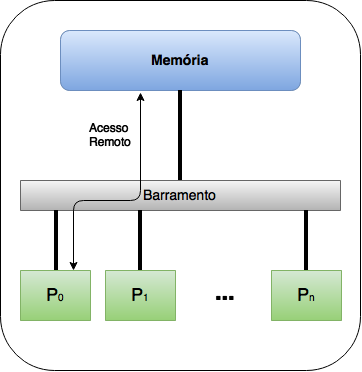
\includegraphics[height=6cm]{images/UMA.png}
}
\subfigure[Arquitetura NUMA]{
  \label{numa_fig}
  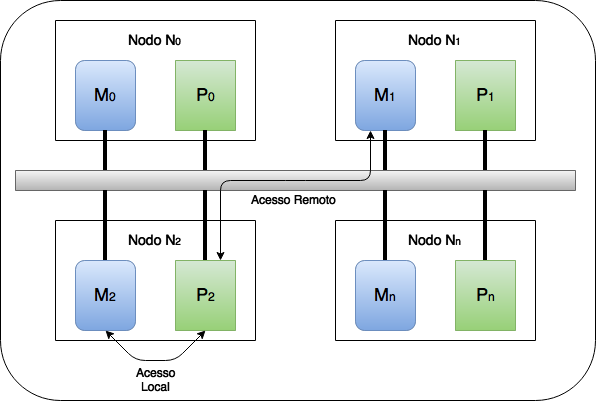
\includegraphics[height=6cm]{images/NUMA.png}
}
\caption{Configuração das arquiteturas UMA e NUMA. Fonte:~\cite{Rodolfo:2014}}
\label{arquiteturas_config}
\end{figure}

O custo não uniforme de acesso à memória é importante para o desempenho de uma aplicação, pois este pode oferecer desvantagens quando não forem avaliados. Uma forma bastante comum de medir a não uniformidade de acessos à memória nas arquiteturas assimétricas, é considerar a razão entre o acesso a uma posição de memória remota e um acesso a uma posição de memória local. Esta razão é denominada fator \emph{NUMA}, uma máquina pode apresentar diferentes valores para o fator \emph{NUMA}, dependendo de quais memórias serão acessadas pelos processadores. Portanto, para que uma aplicação execute de forma eficiente é desejável que os processos sejam escalonados próximos a faixa de endereçamento que eles acessam, assim reduzindo o fator \emph{NUMA}.

É importante conhecer as características da arquitetura \emph{NUMA}, principalmente a latência de acesso às memórias remotas. Estas informações servem de subsidio ao desenvolvedor para que este consiga definir estratégias de escalonamento de tarefas mais eficientes para aplicações que executam neste tipo de arquitetura.


\section{NUMA-Aware}

Arquiteturas \emph{NUMA} apresentam boas características para aplicações com alto nível de paralelismo, porém, os programadores precisam ter cuidado ao escrever códigos para estas arquiteturas. Com isto surgiu o conceito de \emph{NUMA-Aware}, que aborda maneiras para que os programas utilizem com total eficiência os recursos da máquina.

O conceito de \emph{NUMA-Aware} esta relacionado a melhorias em programas, como visto em \cite{mohamedin2016}, pode-se ter melhorias de desempenho a partir gerenciador de contenção que trata conflitos ocorridos entre nodos de forma diferente dos conflitos ocorridos em um único nodo. Também pode-se obter melhor desempenho das arquiteturas com um escalonador de tarefas, no qual o escalonador considera o endereço de memória que a tarefa acessará, assim reduzindo o tempo de leitura e escrita das tarefas executadas pelo programa \cite{blagodurov2010}.


\section{HwLoc}

Para extrair o melhor desempenho de máquinas \emph{NUMA} é necessário conhecer a arquitetura que está sendo utilizada, para obter tais informações de maneira eficiente podemos utilizar o conjuntos de ferramentas \emph{HwLoc~(Hardware Locality)}.

\emph{HwLoc} é um conjunto de ferramentas que possui sua API escrita em linguagem C, esta tem por finalidade obter o mapa hierárquico dos principais elementos presentes na arquitetura de uma máquina, como os níveis de memória \emph{cache}, nodos \emph{NUMA}, soquete, núcleos de processamento e dispositivos de \emph{I/O}.

Esta ferramenta suporta uma variedade de sistemas operacionais e plataformas, além disto, pode agrupar as topologias de várias máquinas em uma única, com a finalidade de permitir que os aplicativos consigam ter uma visão geral da topologia de um conjunto de máquinas, como por exemplo em um \emph{cluster}.

A topologia da máquina compreende todas as informações que podem ser coletadas sobre o \emph{hardware} em que a aplicação está sendo executada, como a localização física de um núcleo de processamento e suas interligações dentro de um determinado processador ou nó de processamento.

As arquiteturas estão tornando-se cada vez mais complexas, com vários níveis de memória \emph{cache}, podendo conter blocos de \emph{cache} específicos (um para cada processador), blocos de \emph{cache} globais (um para todos os processadores) ou ainda alguns blocos de \emph{cache} parcialmente compartilhados (um bloco compartilhado entre alguns processadores).

Estas informações da topologia da máquina precisam ser conhecidas durante a execução do programa para extrair o máximo de desempenho. O \emph{HwLoc} obtém as informações da topologia e as disponibiliza ao programador de diversas maneiras. A topologia da máquina pode ser armazenada em uma representação gráfica ou em outros formatos como texto, xml, pdf, entre outros. Pode ainda ser obtida em tempo de execução com o uso da interface que a ferramenta disponibiliza.

Para obter o máximo possível de informações sobre o \emph{hardware} da máquina, a ferramenta \emph{HwLoc} foi estendida por \cite{Pilla_laercio2014}, para que fornecesse uma visão genérica e completa de qualquer arquitetura de computador. O modelo da arquitetura foi melhorado, passando a oferecer estatísticas de memória, como por exemplo os tempo de latência para buscar dados a partir de diferentes níveis de cache e memória compartilhada e também estatísticas das interconexões, como por exemplo a largura de banda para o tráfego dos dados. Em outras palavras, a ferramenta passou a fornecer informações da distância entre os núcleos de processamento da máquina com base nos tempos de latência nos acessos à memória e largura de banda para a transmissão de dados.

Essas informações são geradas em forma de árvore, a qual é composta pela máquina na raiz e os processadores nas folhas, contendo todos os níveis de cache nos níveis intermediários. As principais vantagens da utilização deste modelo como descrição da topologia da máquina são: (i) modelo genérico, pode ser facilmente calculado por diferentes máquinas e bibliotecas de programação, (ii) agrega as diferentes características de máquinas \emph{multicore}. Além disso, as informações de hierarquia de \emph{cache} e latência de acesso a memória podem ser pré-computadas e armazenadas antes da execução da aplicação, o que reduz o \emph{overhead}, uma vez que elas não precisam ser calculadas novamente toda vez que uma aplicação for executada \cite{Pilla_laercio2014}.


\chapter{Shrink}

...

\chapter{STAMP}
\label{chapter::benchmark}


STAMP~\cite{STAMP} é um conjunto de \emph{benchmarks} criado para pesquisa de memórias transacionais, composto por oito \emph{benchmarks}. Apesar de desenvolvido para a STM~TL2, com algumas modificações disponíveis pode ser usado no \emph{TinySTM}.  A versão do STAMP utilizada será a 0.9.10. O conjunto de \emph{benchmarks} STAMP foi escolhido devido a ele implementar vários \emph{benchmarks}, assim, atingindo uma maior área de aplicações das STM além de ser o conjunto de \emph{benchmark} mais utilizado na pesquisa de STM.


Os \emph{benchmarks} implementados pelo STAMP são~\cite{STAMP}:
\newline


\section{\textbf{Bayes}}

Esta aplicação implementa um algoritmo de aprendizado de redes Bayesianas, que é uma parte importante do aprendizado de máquina. Normalmente, nem as distribuições de probabilidades nem as dependências condicionais entre eles são conhecidas ou podem ser resolvidos por um ser humano, assim redes Bayesianas são frequentemente estudadas com os dados observados. O algoritmo específico implementa uma estratégia de \emph{hill-climbing} ou subida de encosta que usa buscas locais e globais, semelhante à técnica descrita em~\cite{bayesian}. Para estimativas eficientes de distribuição de probabilidade, utiliza-se uma \emph{adtree} ou árvore de decisão a partir de~\cite{Moore97}.


\section{\textbf{Genome}}

Este \emph{benchmark} implementa um programa de sequenciamento de genes que reconstrói a sequência de genes a partir de sequências maiores. O algoritmo usado para o sequenciamento de genes têm  três fases:

\begin{enumerate}
  \item [1.] Remove os segmentos duplicados utilizando uma \emph{hash};
  \item [2.] Combina segmentos utilizando o algoritmo de pesquisa de sequência \emph{Rabin-Karp}~\cite{Karp87}; e
  \item [3.] Constrói a sequência.
  \newline
\end{enumerate}


\section{\textbf{Intruder}}

Este \emph{benchmark} simula o Design 5 dos NIDS~(\emph{Network Intrusion Detection System}) descritos por Haagdorens em~\cite{Haagdorens05}. Pacotes de rede são processados paralelamente e passam por três fases: captação, remontagem e detecção. A estrutura de dados principal na fase de captura é uma simples fila, e a fase de remontagem utiliza um dicionário (implementado por uma árvore auto balanceada), que contém a lista de pacotes que pertencem à mesma seção. Ao avaliar seus cinco designs para um NIDS \emph{multithread}, Haagdorens afirma que a complexidade da fase de remontagem fez com que ele utilize a sincronização de grãos grosso nos designs~4 e~5. Assim, embora estes dois modelos tentam explorar níveis mais elevados de simultaneidade, a sincronização aproximada de grão resulta em um pior desempenho.


\section{\textbf{Kmeans}}

Este \emph{benchmark} foi tirado do \emph{NU-MineBench 2.0}~\cite{Pisharath05}. \emph{K-means} é um método baseado em partição~\cite{Bezdek81} e é sem dúvida a técnica de agrupamento mais utilizada. Este algoritmo é comumente usado para partição de itens de dados em subconjuntos relacionados. Cada \emph{thread} processa uma partição dos objetos iterativamente. A versão transacional adiciona uma transação para proteger o update do centro do \emph{cluster} que ocorre durante cada iteração.


\section{\textbf{Labyrinth}}

Dado um labirinto, este \emph{benchmark} encontra os caminhos de menor distância entre os pares de pontos inicial e final. O algoritmo de roteamento utilizado é o algoritmo Lee~\cite{Lee61}.

Nesse algoritmo, o labirinto é representado como uma grade, em que cada ponto de grade pode conter ligações adjacentes, para os pontos da grade que não estão nas diagonais. O algoritmo busca um caminho mais curto entre os pontos de conexão através da realização de uma busca em largura e marca cada ponto da grade com a sua distância para o início. Esta fase de expansão acabará por chegar ao ponto final, se a conexão for possível. A segunda fase de rastreamento, em seguida, estabelece a ligação, seguindo todo o caminho diminuindo a distância. Este algoritmo é garantido para encontrar o caminho mais curto entre um ponto inicial e final, no entanto, quando vários caminhos são feitos, um caminho pode bloquear outro.


\section{\textbf{SSCA2}}

\emph{Scalable Synthetic Compact Applications 2}~(SSCA2)~\cite{Bader05} é composta por quatro \emph{kernels} que operam em um grande, dirigido e ponderado gráfico. Estes quatro \emph{kernels} gráficos são comumente usados em aplicações que vão desde a biologia computacional até a segurança. STAMP incide sobre um \emph{Kernel}, que constrói uma estrutura de dados eficiente utilizando matrizes de adjacência e matrizes auxiliares.


\section{\textbf{Vacation}}

Este \emph{benchmark} implementa um sistema de reserva de viagens alimentado por um banco de dados não-distribuído. A carga de trabalho é composto por vários segmentos de clientes que interagem com o banco de dados via gerenciador de transações do sistema.

O banco de dados é composto por quatro tabelas: carros, quartos, voos e clientes. Os três primeiros têm relações com os campos que representam um número único de identificação, quantidade reservada, a quantidade total disponível, e preço. A tabela de clientes acompanha as reservas feitas por cada cliente e o preço total das reservas que eles fizeram. As tabelas são implementados como árvores rubro negras.


\section{\textbf{Yada}}

Este \emph{benchmark} implementa o algoritmo de Ruppert para refinamento de malha~\cite{Ruppert95}. A versão transacional é similar em design ao apresentado em~\cite{Kulkarni06}.

\chapter{Metodologia}

...

\chapter{Desenvolvimento}

  ...

\begin{figure}[htbp]
  \centering 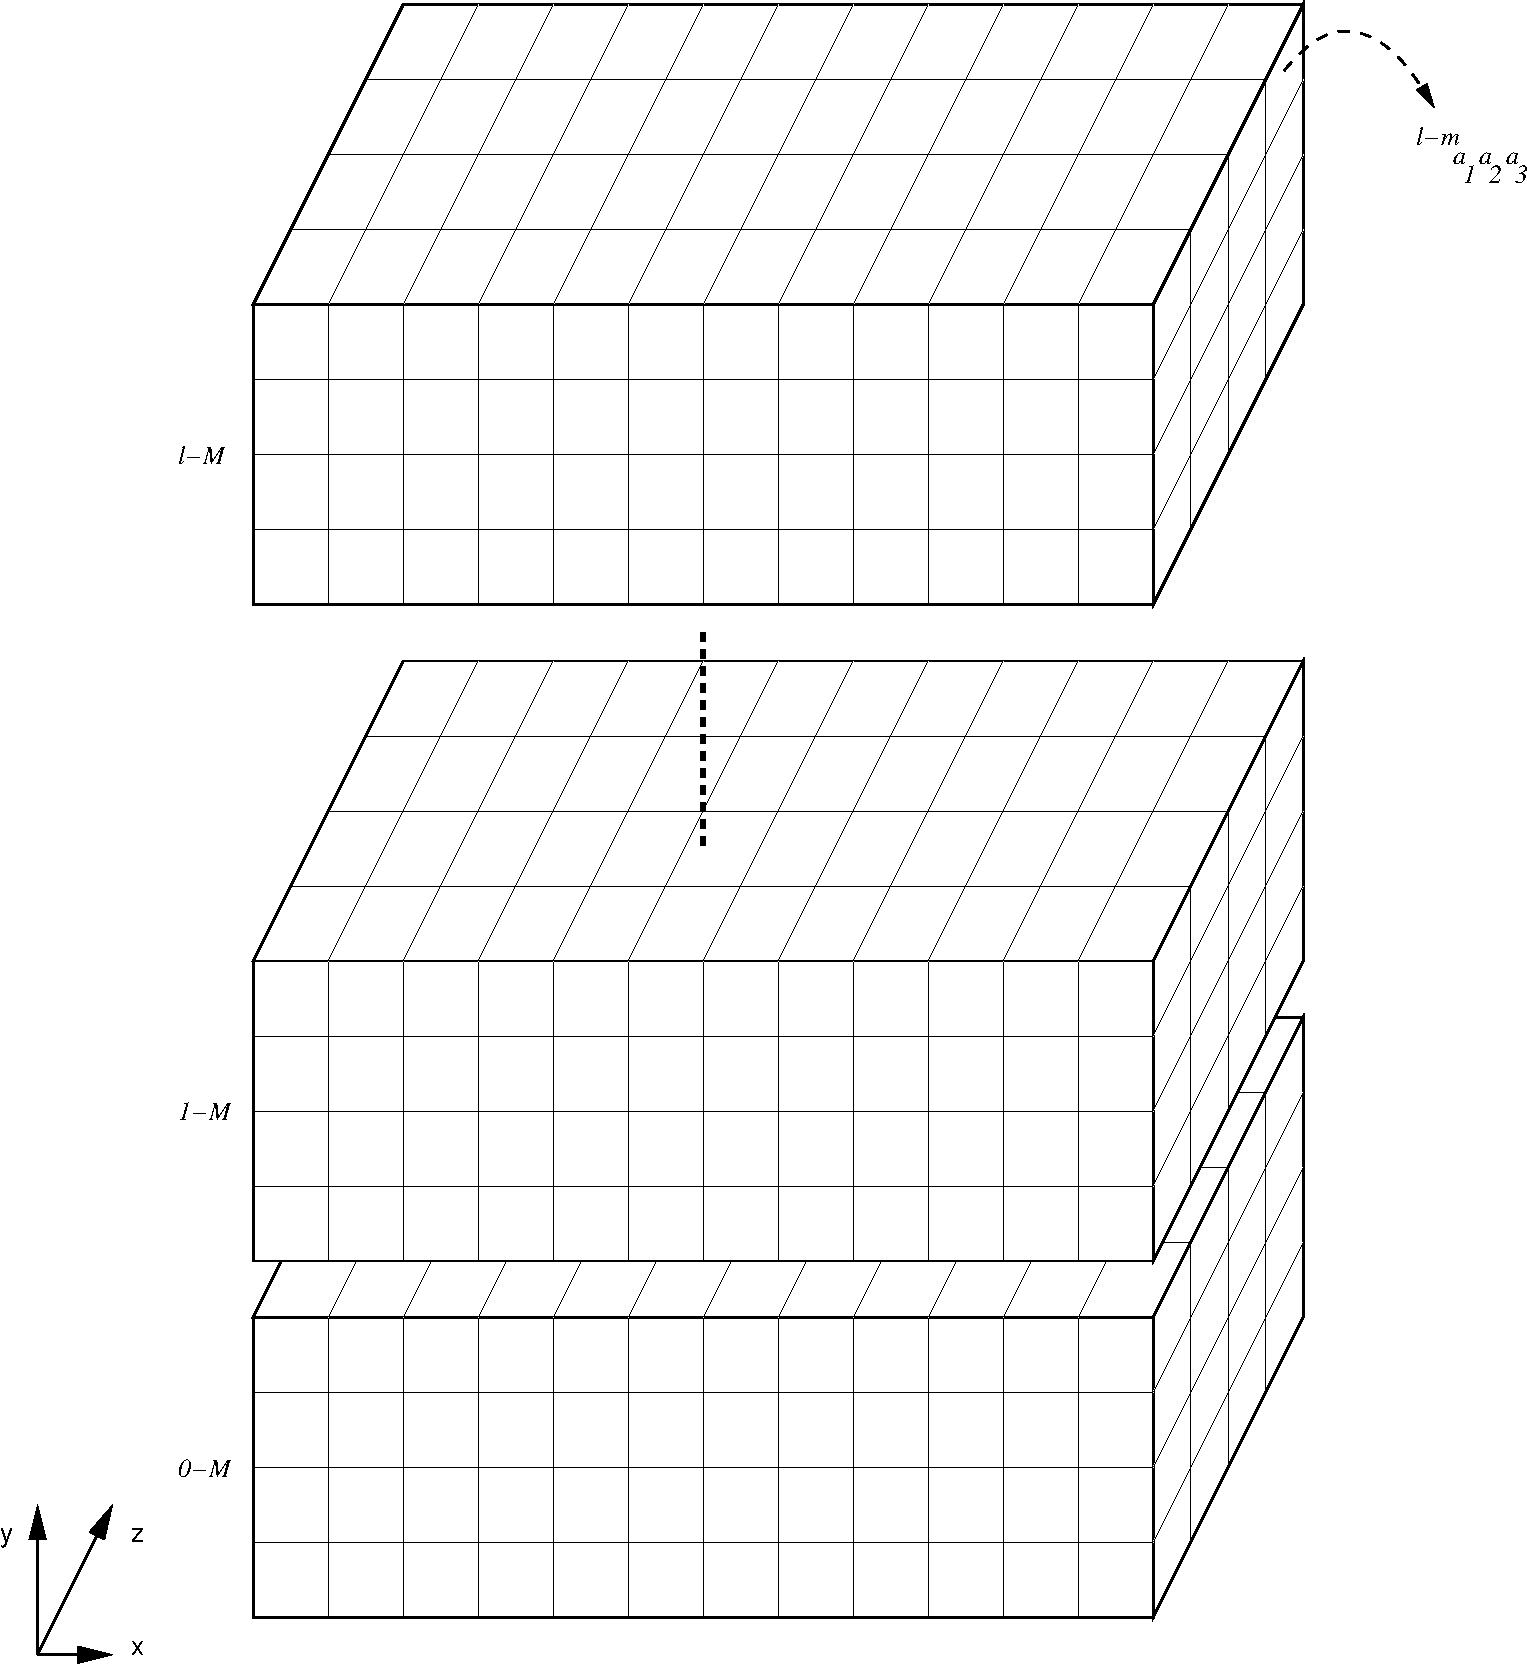
\includegraphics[scale=.4]{images/figura}
\caption{Nome da figura} 
\label{figura}
\end{figure}


\section{\textbf{Lstm}}

O escalonador desenvolvido denominado Lstm é dividido em três etapas. As etapas são inicialização do sistema, execução e coleta de dados, e migração das threads em execução.

A primeira etapa, inicialização do sistema, como o nome sugere ocorre no inicio da aplicação e é responsavel por identificar a arquitetura utilizada, montar as filas de execução e distribuir as threads entre estás filas.

No inicio destá etapa o escalonador lê a arquitetura utilizada para saber a quantidade de cores disponivel na arquitetura, se o número de thread solicitado pela aplicação for menor que o número de cores disponivel na arquitetura o escalonador cria uma fila de execução para cada thread solicitada.  Se o número de threads solicitados for maior que o número de cores da arquitetura, é criada uma fila de execução para cada core da arquitetura.

Após as filas de execução serem criadas, o escalonador se encarrega de distribuir com base em uma heuristica esses threads recem criados entre as filas de execução. Temos duas heurísticas utilizadas para distribuição das threads entre as filas.

A primeira heuristica de distribuição resumese a distribuir de forma ordenada uma thread para cada fila de execução, repetindo a distribuição caso haja mais threads do que filas...

A segunda heuristica de distribuição resumese a distribuir de forma ordenada duas threads para cada fila de execução, repetindo a distribuição caso haja mais threads do que filas...

Na segunda etapa a aplicação é realizada, cada thread pode ter n transações. Nessa etapa o escalonador utiliza os recursos desenvolvidos em STmap para coletar as informações sobre as transações executadas nessas threads.

Aqui é montada a matriz de comunicação que indica o indice de leitura e escrita uma thread possui em relação as demais. Também coletamos as informações sobre o indice de commits e aborts realizados por thread e montamos a matriz com os ultimos endereços de memória acessados pelas threads.

A terceira etapa só é executada se uma transação abortar. Nesta etapa avaliamos para qual fila a thread em execução pode ser migrada, e utilizamos uma heuristica para tomar a decisão de migrar a thread de sua fila de execução para outra fila.

No momento do abort consultamos a matriz de comunicação previamente montada para descobrir com qual outra thread temos um maior número de leitura e escrita em comum. Após descobrir qual é esta thread utilizamos esse valor para descobrir qual sua fila de execução atual, é para esta fila que o escalonador poderá efetuar a migração.

Caso a thread atual não esteja na mesma fila que a outra thread o escalonador avalia a possibilidade de migração desta thread. Para tomar a decisão de executar ou não a migração foi implementada duas heurísticas distintas. A primeira chamada latency tem como base avaliar a latencia de acesso à memória, a segunda denominada treshold avalia a relação entre commits e aborts existentes na thread em execução.

Para realizar a heuristica latency primeiro consultamos a matriz com o endereço de memória do ultimo acesso em comum entre as duas threads e então consultamos a qual região de memória esse endereço pertence. Após isto é coletada a informação de qual nodo a fila que a thread esta executando pertence e qual nodo pertence a fila que receberá o thread.

Se a latencia entre a fila atual e posição de memória for maior que a latencia entre a nova fila e a posição de memória o escalonador se encarrega de adormecer a thread atual e migrar ela para nova fila de execução.

Para executar a heuristica treshold o escalonador avalia qual a diferença entre abort e commit existente na thread em execução. Caso o valor da diferença fique acima de um limiar estipulado o escalonador se encarrega de adormecer a thread em execução e migrala para nova fila.

Após a heuristica ser executada e a migração ter sido realizada, o escalonador avalia se existe mais threads disponiveis para execução na fila de execução. Se a migração não for executada a execução da thread prosegue realizando um processo de abort padrão da biblioteca de stm.


\chapter{Conclusão}

...

\section{Resultados}

...

% Bibliografia http://liinwww.ira.uka.de/bibliography/index.html um
% site que cataloga no formato bibtex a bibliografia em computacao
% \bibliography{nomedoarquivo.bib} (sem extensao)
% \bibliographystyle{formato.bst} (sem extensao)

\bibliographystyle{abnt}
\bibliography{bibliografia} 

% Apêndices (Opcional) - Material produzido pelo autor
\apendices
\chapter{Um Apêndice}

% Anexos (Opcional) - Material produzido por outro
\anexos
\chapter{Um Anexo}

...

\chapter{Outro Anexo}

...

% Faz a capa do CDROM
% \makecover

\end{document}

